\documentclass[10pt, dvipdfmx]{beamer}

\renewcommand{\kanjifamilydefault}{\gtdefault}
%%%%%%%%%%%  package  %%%%%%%%%%%
\usepackage{bxdpx-beamer}% dvipdfmxなので必要
\usepackage{pxjahyper}% 日本語で'しおり'したい

\usepackage{amssymb,amsmath,ascmac}

\usepackage{multirow}
\usepackage{bm}

\graphicspath{{../Figures/Rheology/}{../Figures/adhesives/}}

\usepackage{tikz}
\usepackage{xparse}
\usetikzlibrary{shapes,arrows}
%% define fancy arrow. \tikzfancyarrow[<option>]{<text>}. ex: \tikzfancyarrow[fill=red!5]{hoge}
\tikzset{arrowstyle/.style n args={2}{inner ysep=0.1ex, inner xsep=0.5em, minimum height=2em, draw=#2, fill=black!20, font=\sffamily\bfseries, single arrow, single arrow head extend=0.4em, #1,}}
\NewDocumentCommand{\tikzfancyarrow}{O{fill=black!20} O{none}  m}{
\tikz[baseline=-0.5ex]\node [arrowstyle={#1}{#2}] {#3 \mathstrut};}
%
%微分関連のマクロ
%
\newcommand{\diff}{\mathrm d}
\newcommand{\difd}[2]{\dfrac{\diff #1}{\diff #2}}
\newcommand{\difp}[2]{\dfrac{\partial #1}{\partial #2}}
\newcommand{\difdd}[2]{\dfrac{\diff^2 #1}{\diff #2^2}}
\newcommand{\difpp}[2]{\dfrac{\partial^2 #1}{\partial #2^2}}

%目次スライド
\AtBeginSection[]{
  \frame{\tableofcontents[currentsection]}
}
%アペンディックスのページ番号除去
\newcommand{\backupbegin}{
\newcounter{framenumberappendix}
\setcounter{framenumberappendix}{\value{framenumber}}
}
\newcommand{\backupend}{
\addtocounter{framenumberappendix}{-\value{framenumber}}
\addtocounter{framenumber}{\value{framenumberappendix}} 
}

%%%%%%%%%%%  theme  %%%%%%%%%%%
\usetheme{Copenhagen}
% \usetheme{Metropolis}
% \usetheme{CambridgeUS}
% \usetheme{Berlin}

%%%%%%%%%%%  inner theme  %%%%%%%%%%%
% \useinnertheme{default}

% %%%%%%%%%%%  outer theme  %%%%%%%%%%%
\useoutertheme{default}
% \useoutertheme{infolines}

%%%%%%%%%%%  color theme  %%%%%%%%%%%
%\usecolortheme{structure}

%%%%%%%%%%%  font theme  %%%%%%%%%%%
\usefonttheme{professionalfonts}
%\usefonttheme{default}

%%%%%%%%%%%  degree of transparency  %%%%%%%%%%%
%\setbeamercovered{transparent=30}

% \setbeamertemplate{items}[default]

%%%%%%%%%%%  numbering  %%%%%%%%%%%
% \setbeamertemplate{numbered}
\setbeamertemplate{navigation symbols}{}
\setbeamertemplate{footline}[frame number]


\title{降伏挙動について}
\author[東亞合成 佐々木]{佐々木 裕}
\institute[東亞合成]{東亞合成株式会社}
\date{\today}

\begin{document}

%%%%%
% 1 P
%%%%%
\maketitle

%%%%%
% 2 P
%%%%%
%% 目次 (必要なければ省略)
\begin{frame}
\frametitle{Outline}
\tableofcontents
\end{frame}

%%%%%%%%%%%%%%%%%%
\section{やりたいこと}

\subsection{やりたいこと}

\begin{frame}
	\frametitle{やりたいこと}
	\Large
	\begin{itemize}
		\item 物質の強さの発現機構について、もっと知りたい。
		\item 適切なモデル化で、破壊について検討したい。
		\begin{itemize}
			\item 変形時のエネルギー散逸についても知りたい。
			\item 実実験との比較で、降伏挙動をもっと知りたい。
			\item 高分子材料のヤング率についても。
		\end{itemize}
	\end{itemize}
\end{frame}

%%%%%%%%%%%%%%%%%%%
\subsection{単純なモデルの利用}
%%%%%%%%%%%%%%
\begin{frame}\frametitle{単純化した簡単なモデル}

\large
\begin{alertblock}{自然の採る道は単純なこと「も」多い}
\begin{itemize}
%	\large
	\item
	最小作用の原理
	\item
	フェルマーの原理、シュネルの法則
\end{itemize}
\end{alertblock}
\pause
\begin{exampleblock}{テクニカルには}
\begin{itemize}
		\item
		仮想仕事の原理、変分原理
			\begin{itemize}
			\large
			\item
			最速降下問題
			\item
			解析力学でハミルトニアンで議論
			\end{itemize}
		\item
		経路積分
			\begin{itemize}
			\large
			\item
			量子系の運動記述
			\item
			(応用)ポリマーの形態エントロピー
			\end{itemize}
\end{itemize}
\end{exampleblock}
\end{frame}
%%%%%	
\subsection{シミュレーションの利用}
%%%%%%
\begin{frame}\frametitle{シミュレーションの有効性}
\large
\begin{itemize}
	\item
	理想化した議論
	\large
	\begin{itemize}
		\large
		\item
		数学的モデルとの整合性
		\item
		ポテンシャル場: 状態量、エネルギー	
		\item
		熱力学的な平衡状態も仮定しやすい
	\end{itemize}
	\item
	モデル化の条件や領域が明確
	\begin{itemize}
		\large
		\item
		境界条件: ノイマン、デリクレ、周期等
		\item
		拘束条件:NPT等のアンサンブル
	\end{itemize}
	\item
	シミュレーションの方法
	\begin{itemize}
		\large
		\item
		MD:ニュートン力学で粒子化
		\item
		濃度場SCF:ポリマー濃度場を密度汎関数		
	\end{itemize}
\end{itemize}
\end{frame}
%%%%%
\begin{frame}\frametitle{シミュレーションの有効性}
\LARGE

\begin{alertblock}{逆に言えば、}
実事象と合わないときは。
\begin{itemize}
	\item
	理想化のやり方が悪い
	\item
	モデル化の条件や領域が不適切
	\item
	シミュレーションの選択が\\良くない
\end{itemize}
\end{alertblock}
\end{frame}
%%%%%
%%%%%
\begin{frame}\frametitle{物理モデリングとシミュレーション}
	\begin{block}{最近のシミュレーションのトレンド}
	\begin{itemize}
		\item 大規模計算(異なる階層を一気に)
		\item 詳細構造(フルアトミスティック)
	\end{itemize}
大量の計算資源を必要とし、Project化。
	\end{block}

	\begin{alertblock}{私のやりたいこと}
	\begin{itemize}
		\item 注目する事象のターゲットを明確にした
		\item 的確な物理モデルの構築
		\item 容易に実行可能な安価なシミュレーション
		\begin{itemize}
			\item 適正なレベルで粗視化必要十分な大きさのシステム
		\end{itemize}
	\end{itemize}
	\end{alertblock}
\pause
\LARGE
\textcolor{red}{実事象とのバリデーションが重要}
\end{frame}

\section{バルクの破壊}

%%%%%%%%%%%%%%%%%%%%%%
\subsection{固体バルクの力学応答}
%%%%%%%%%%%%%%
\begin{frame}
\frametitle{一般的な応力 - 歪み曲線}

\begin{columns}[totalwidth=1\textwidth]
\column{.6\textwidth}
	\begin{itemize}
	\item 線形領域(~弾性限界):
		\begin{itemize}
		\item この段階までの変形は可逆
		\item {\color{red}「内部構造は変化しない」}
		\end{itemize}
	\item 弾性限界から降伏点:
		\begin{itemize}
		\item 直線から外れて応力が極大
		\item {\color{blue}「不可逆な内部構造の変化が\\生じはじめる」}
		\end{itemize}
	\item 降伏点以降:
		\begin{itemize}
		\item 塑性変形が進行し、破断
		\item 破断点近傍で、{\color{red}「局所的な高分子鎖の切断$\Rightarrow$マクロな破壊」}
		\end{itemize}
	\end{itemize}
%}
\column{.39\textwidth}
%\vspace{-20mm}
	\begin{figure}
	\centering
	
\includegraphics[width=50mm]{S_S_Curve.png}
	\end{figure}
\end{columns}
\end{frame}
%%%%
\subsection{破壊のモード}
\begin{frame}
\frametitle{脆性破壊と延性破壊}

\begin{columns}[totalwidth=1\textwidth]
\column{.5\textwidth}
	\begin{itemize}
	\item 脆性破壊:
		\begin{itemize}
		\item 
		弾性限界を超えると、
		\item
		巨視的な亀裂が生じ、
		\item
		分離し破壊
		\end{itemize}
	\item 延性破壊:
		\begin{itemize}
		\item 
		降伏点が存在し、
		\item
		降伏歪以上でも、
		\item
		延性を示す
		\end{itemize}
	\end{itemize}
%}
\column{.49\textwidth}
%\vspace{-20mm}
	\begin{figure}
	\centering
	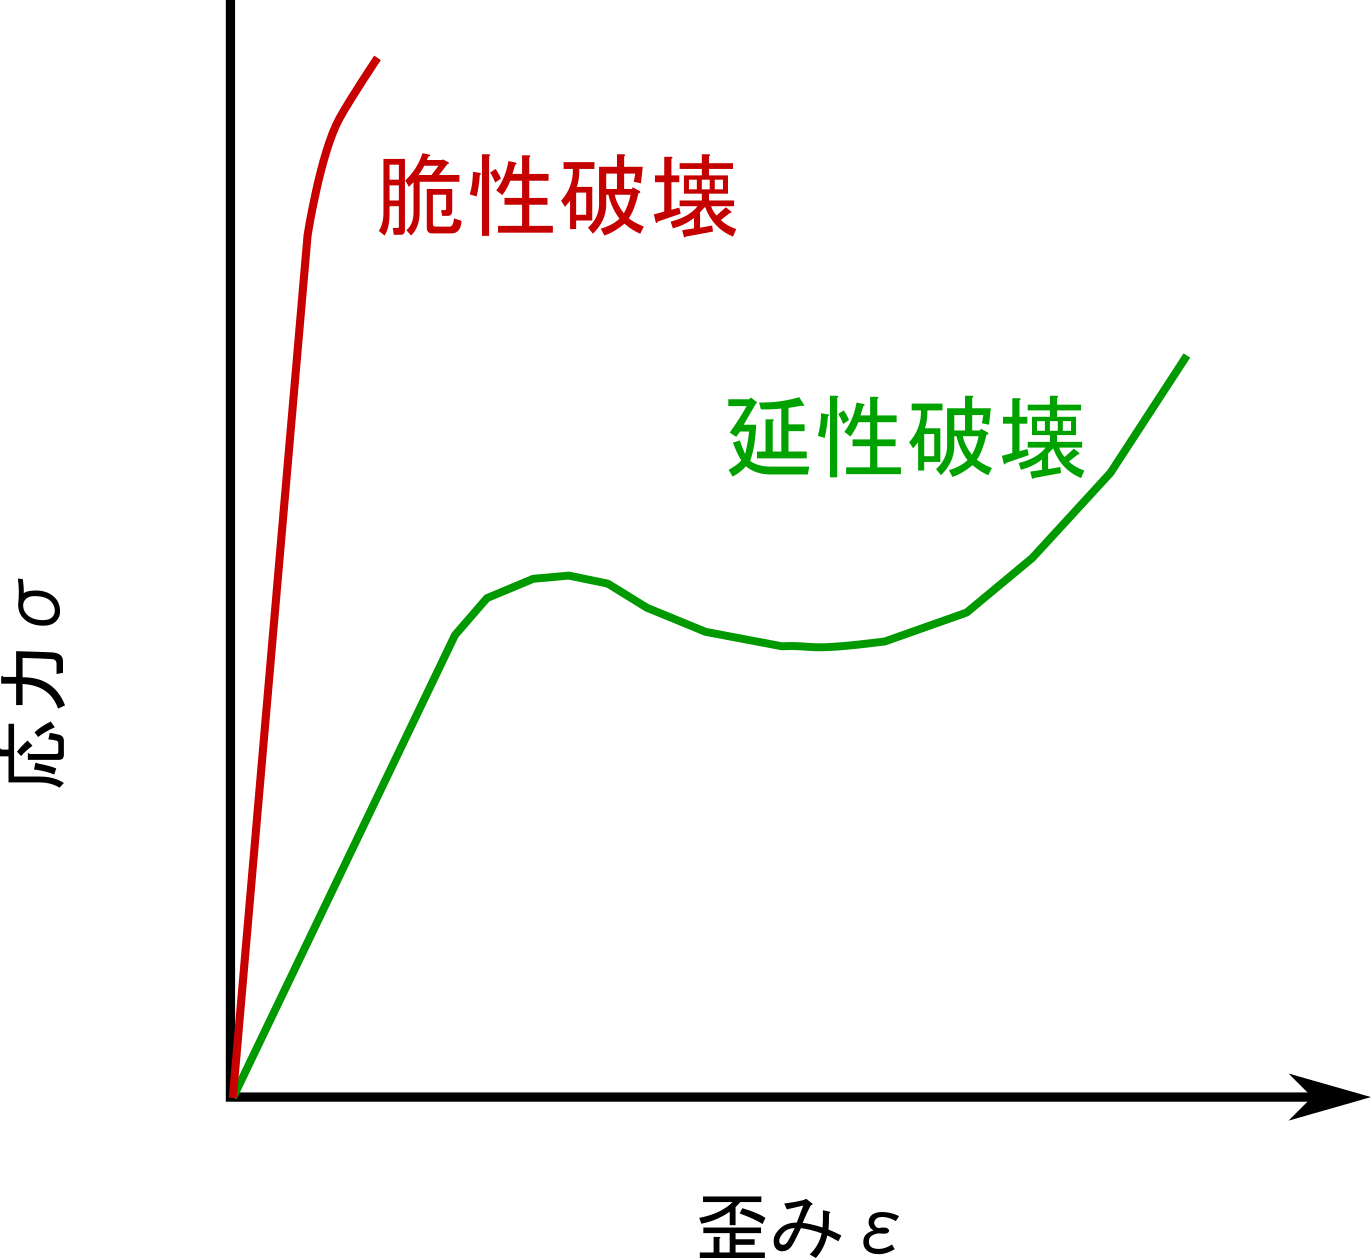
\includegraphics[width=50mm]{S_S_Curve_2.png}
	\end{figure}
\end{columns}

\begin{description}
\item[塑性変形]
弾性限界を超えた外力の印加により生じた歪みのうち、除荷後にも残る永久歪み。
\item[脆性および延性破壊]
主として、塑性変形時に発生する破壊。
\end{description}
\end{frame}

\subsection{破壊工学の考え方}

%%%%%%%%%%%%%%%%%%%%%%%%%%%%%%
\begin{frame}
\frametitle{破壊工学の考え方}
\begin{exampleblock}{系中にクラックが存在することを前提に}

\begin{itemize}
\item
\alert{「クラック近傍での応力集中を如何に抑制するか」}
\end{itemize}
\end{exampleblock}

\begin{columns}[totalwidth=1\textwidth]
\column{.5\textwidth}
\begin{alertblock}{マクロとミクロをつなげると}
	\begin{itemize}
		\item
		\alert{応力拡大係数 $K_I$ で評価}
		\footnotesize
		\begin{align*}
		K_{I} = \sigma \sqrt{\pi c}
		\end{align*}
		\normalsize
		\item 
		クラック進展の抑制 \\
		$\Rightarrow$ 先端での\alert{局所降伏}\\
		降伏応力 $\sigma_Y$ に反比例
		\footnotesize
		\begin{align*}
		d \propto \left( \dfrac{K_I}{\sigma_Y} \right)^2
		\end{align*}
		\normalsize
	\end{itemize}
\end{alertblock}
\column{.5\textwidth}
	\centering
	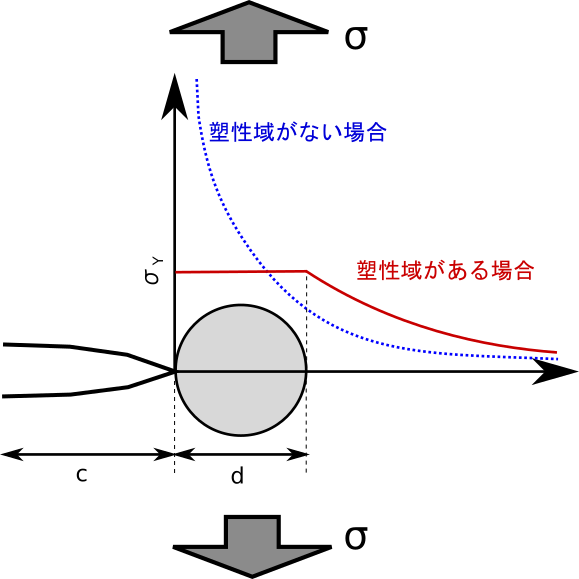
\includegraphics[width=.9\textwidth]{yeild_crack.png}
\end{columns}
\end{frame}

%%%%%%%%%%%%%%%
\begin{frame}
%[shrink squeeze]
\frametitle{降伏挙動と破壊モード}
\begin{columns}[totalwidth=1\textwidth]
\column{.5\textwidth}
ガラス状態の高分子材料では、
\begin{block}{破壊のモード(巨視的)}
脆性破壊 $\Leftrightarrow$ 延性破壊\\
脆性破壊は、降伏前にミクロなクラックが進展した破壊とも考えられる。
\end{block}
\column{.5\textwidth}
	\centering
	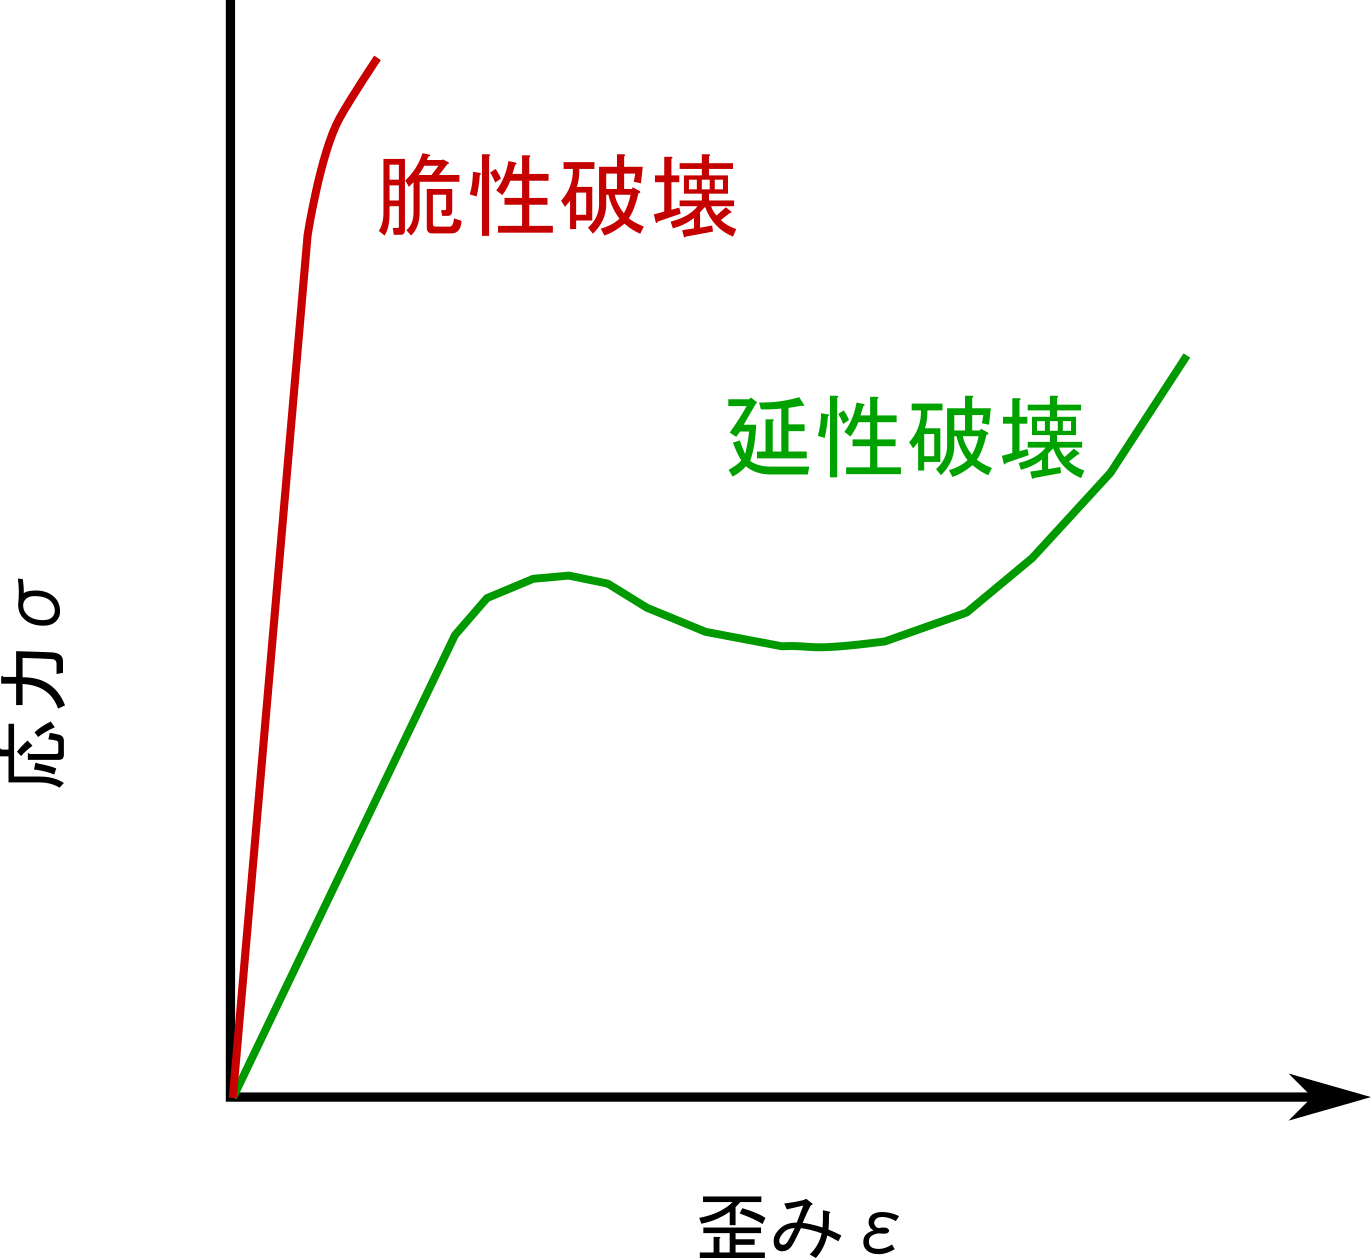
\includegraphics[width=.9\textwidth]{S_S_Curve_2.png}
\end{columns}
\begin{exampleblock}{延性破壊モードにするために}
	\begin{itemize}
		\item
		{\color{red} 局所的な降伏}が必須。
		\item
		クレイズのような局所的な破壊も含む
		\item 
		一般に、高分子材料の{\color{red} 降伏は不可逆}。
	\end{itemize}
\end{exampleblock}
\end{frame}


\section{降伏挙動}
\subsection{液体の微視的モデル}
%%%%%%%%%%%%%%%%%%%%%%%%%%%
\begin{frame}
\frametitle{液体の微視的モデル}

\begin{figure}
 \centering
	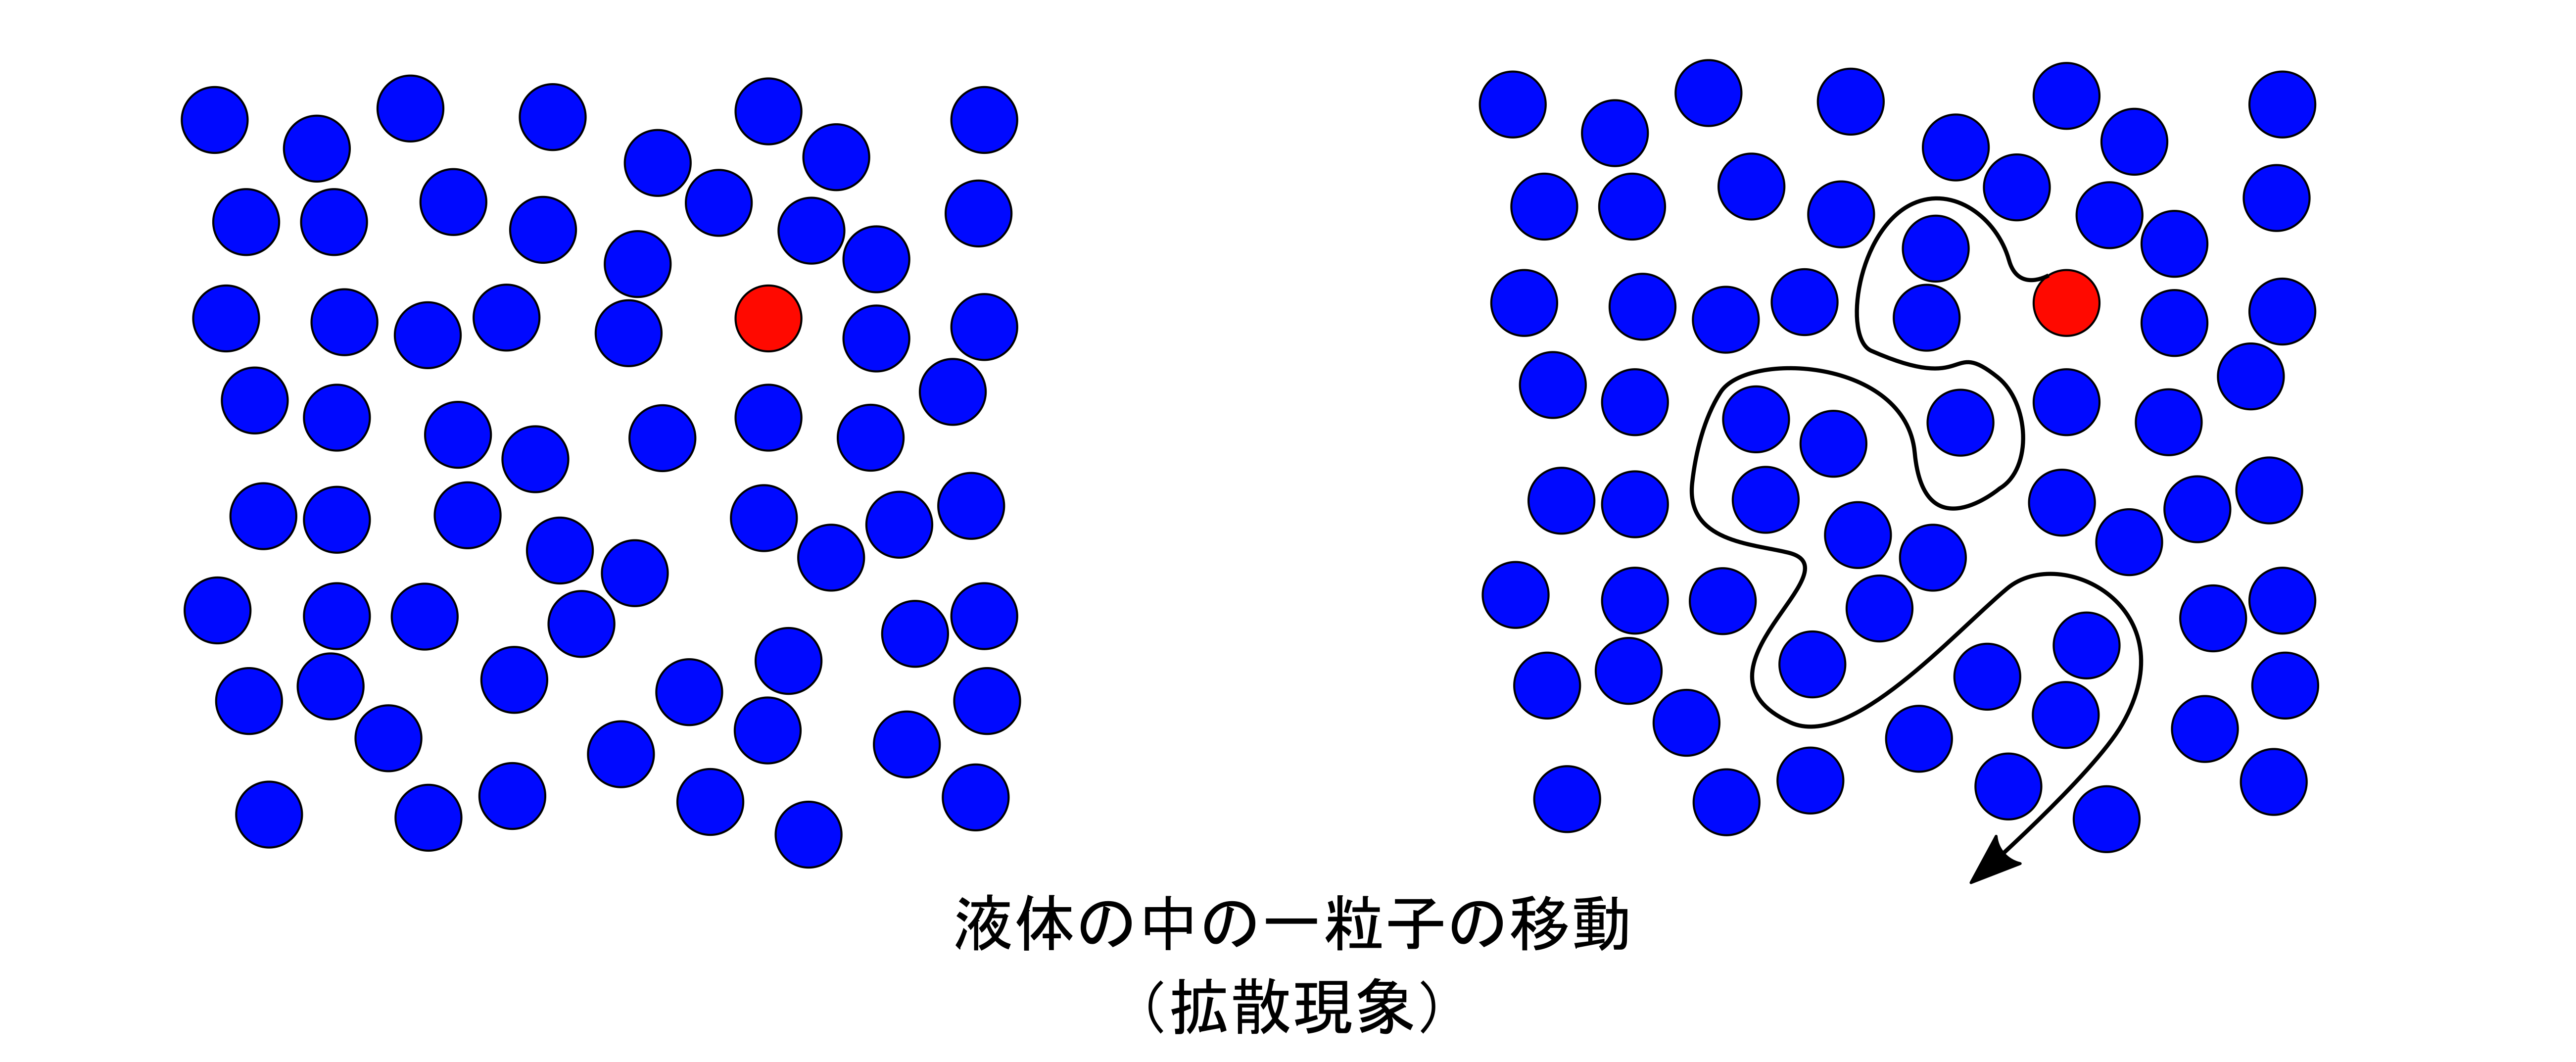
\includegraphics[width=\textwidth]{liquid_1.png}
%	\caption{•}
%	\label{fig: •}
\end{figure}
\end{frame}

%%%%%%%%%%%%%%%%%%%%%%%%%%%
\begin{frame}
	\frametitle{変形付与時の粒子の移動}
	
	\begin{figure}
	 \centering
		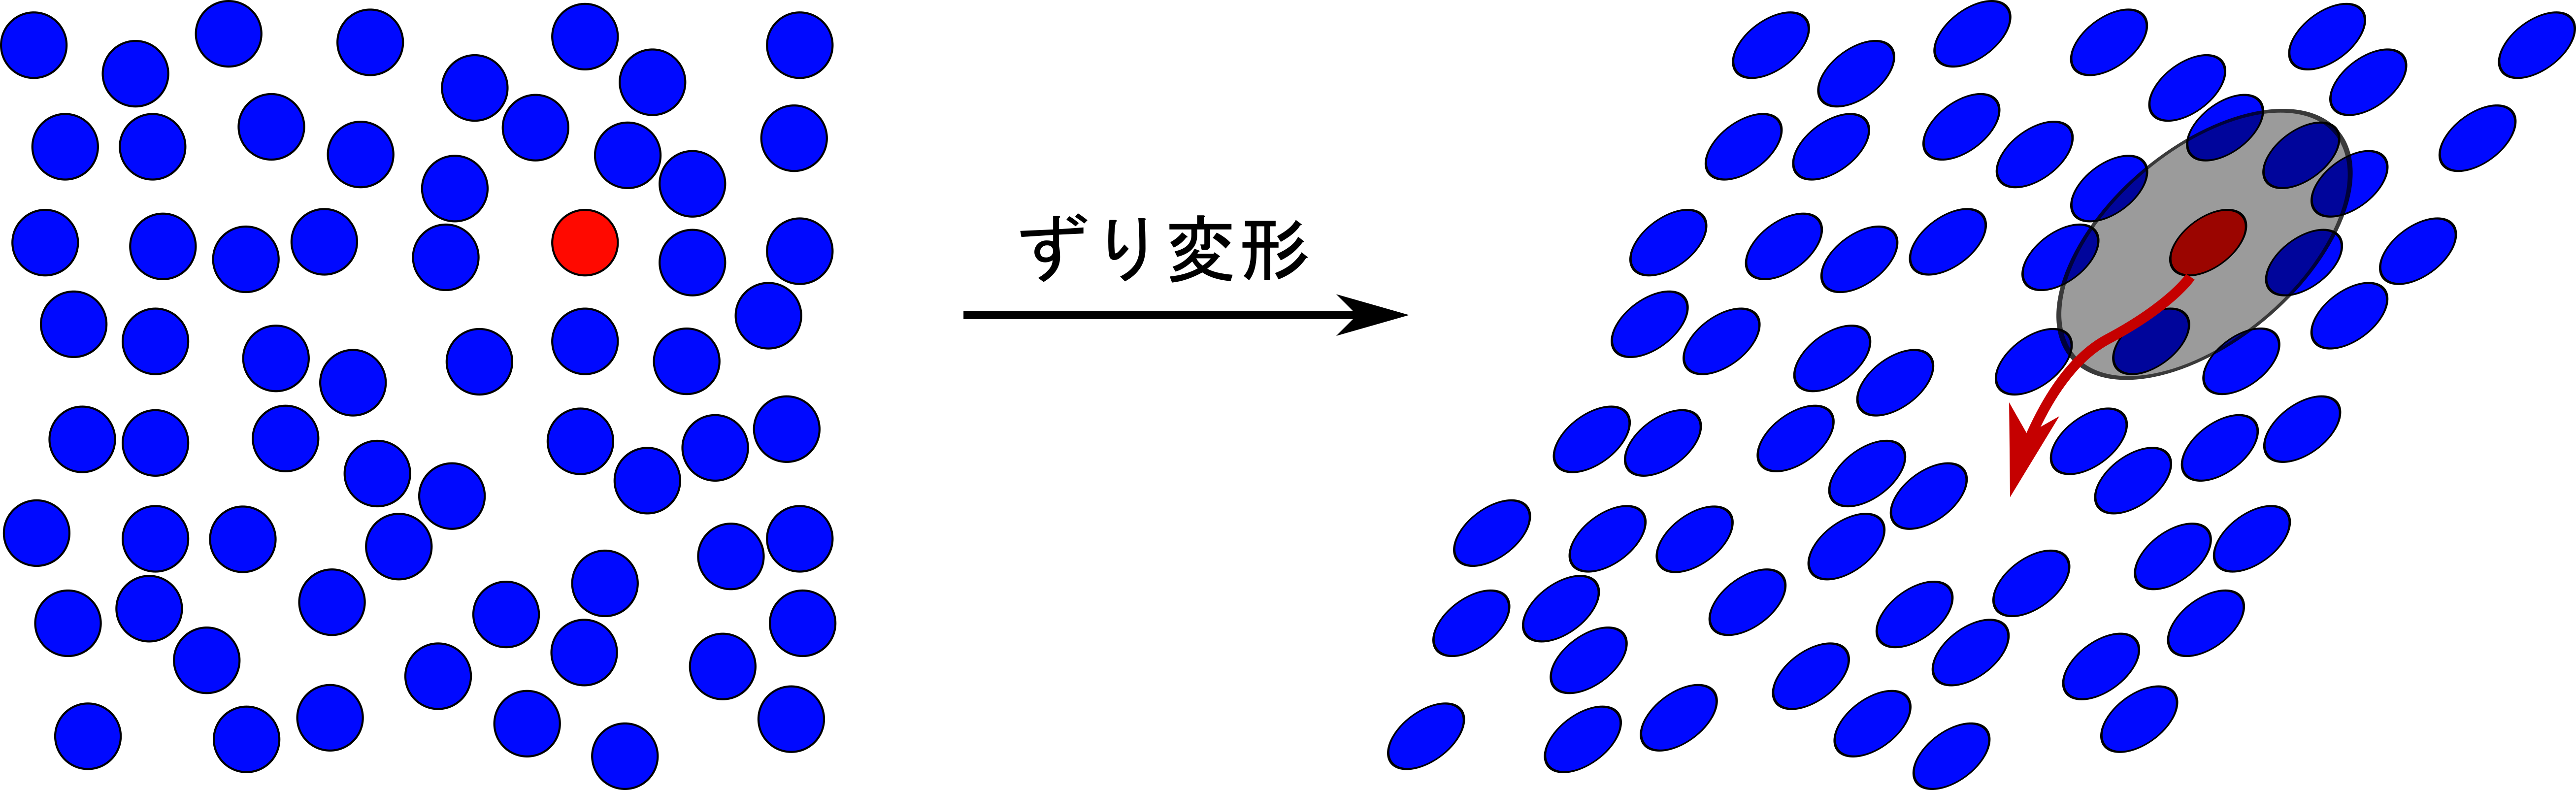
\includegraphics[width=\textwidth]{liquid_flow.png}
	%	\caption{•}
	%	\label{fig: •}
	\end{figure}
	\end{frame}

%%%%%%%%%%%%%%%%%%%%%%%%%%%
\begin{frame}
\frametitle{Eyring の流動モデル}

\begin{itemize}
\item 活性化エネルギー($\Delta G$)の山を超えて、粒子が移動
\item 応力がなければ、両方向の移動が同一
\item 応力印加により、移動の不均一(流動)
\item 応力に粒子が占める体積(のようなもの)$v^*$ を乗じてエネルギーの次元
\end{itemize}

\begin{figure}
 \centering
	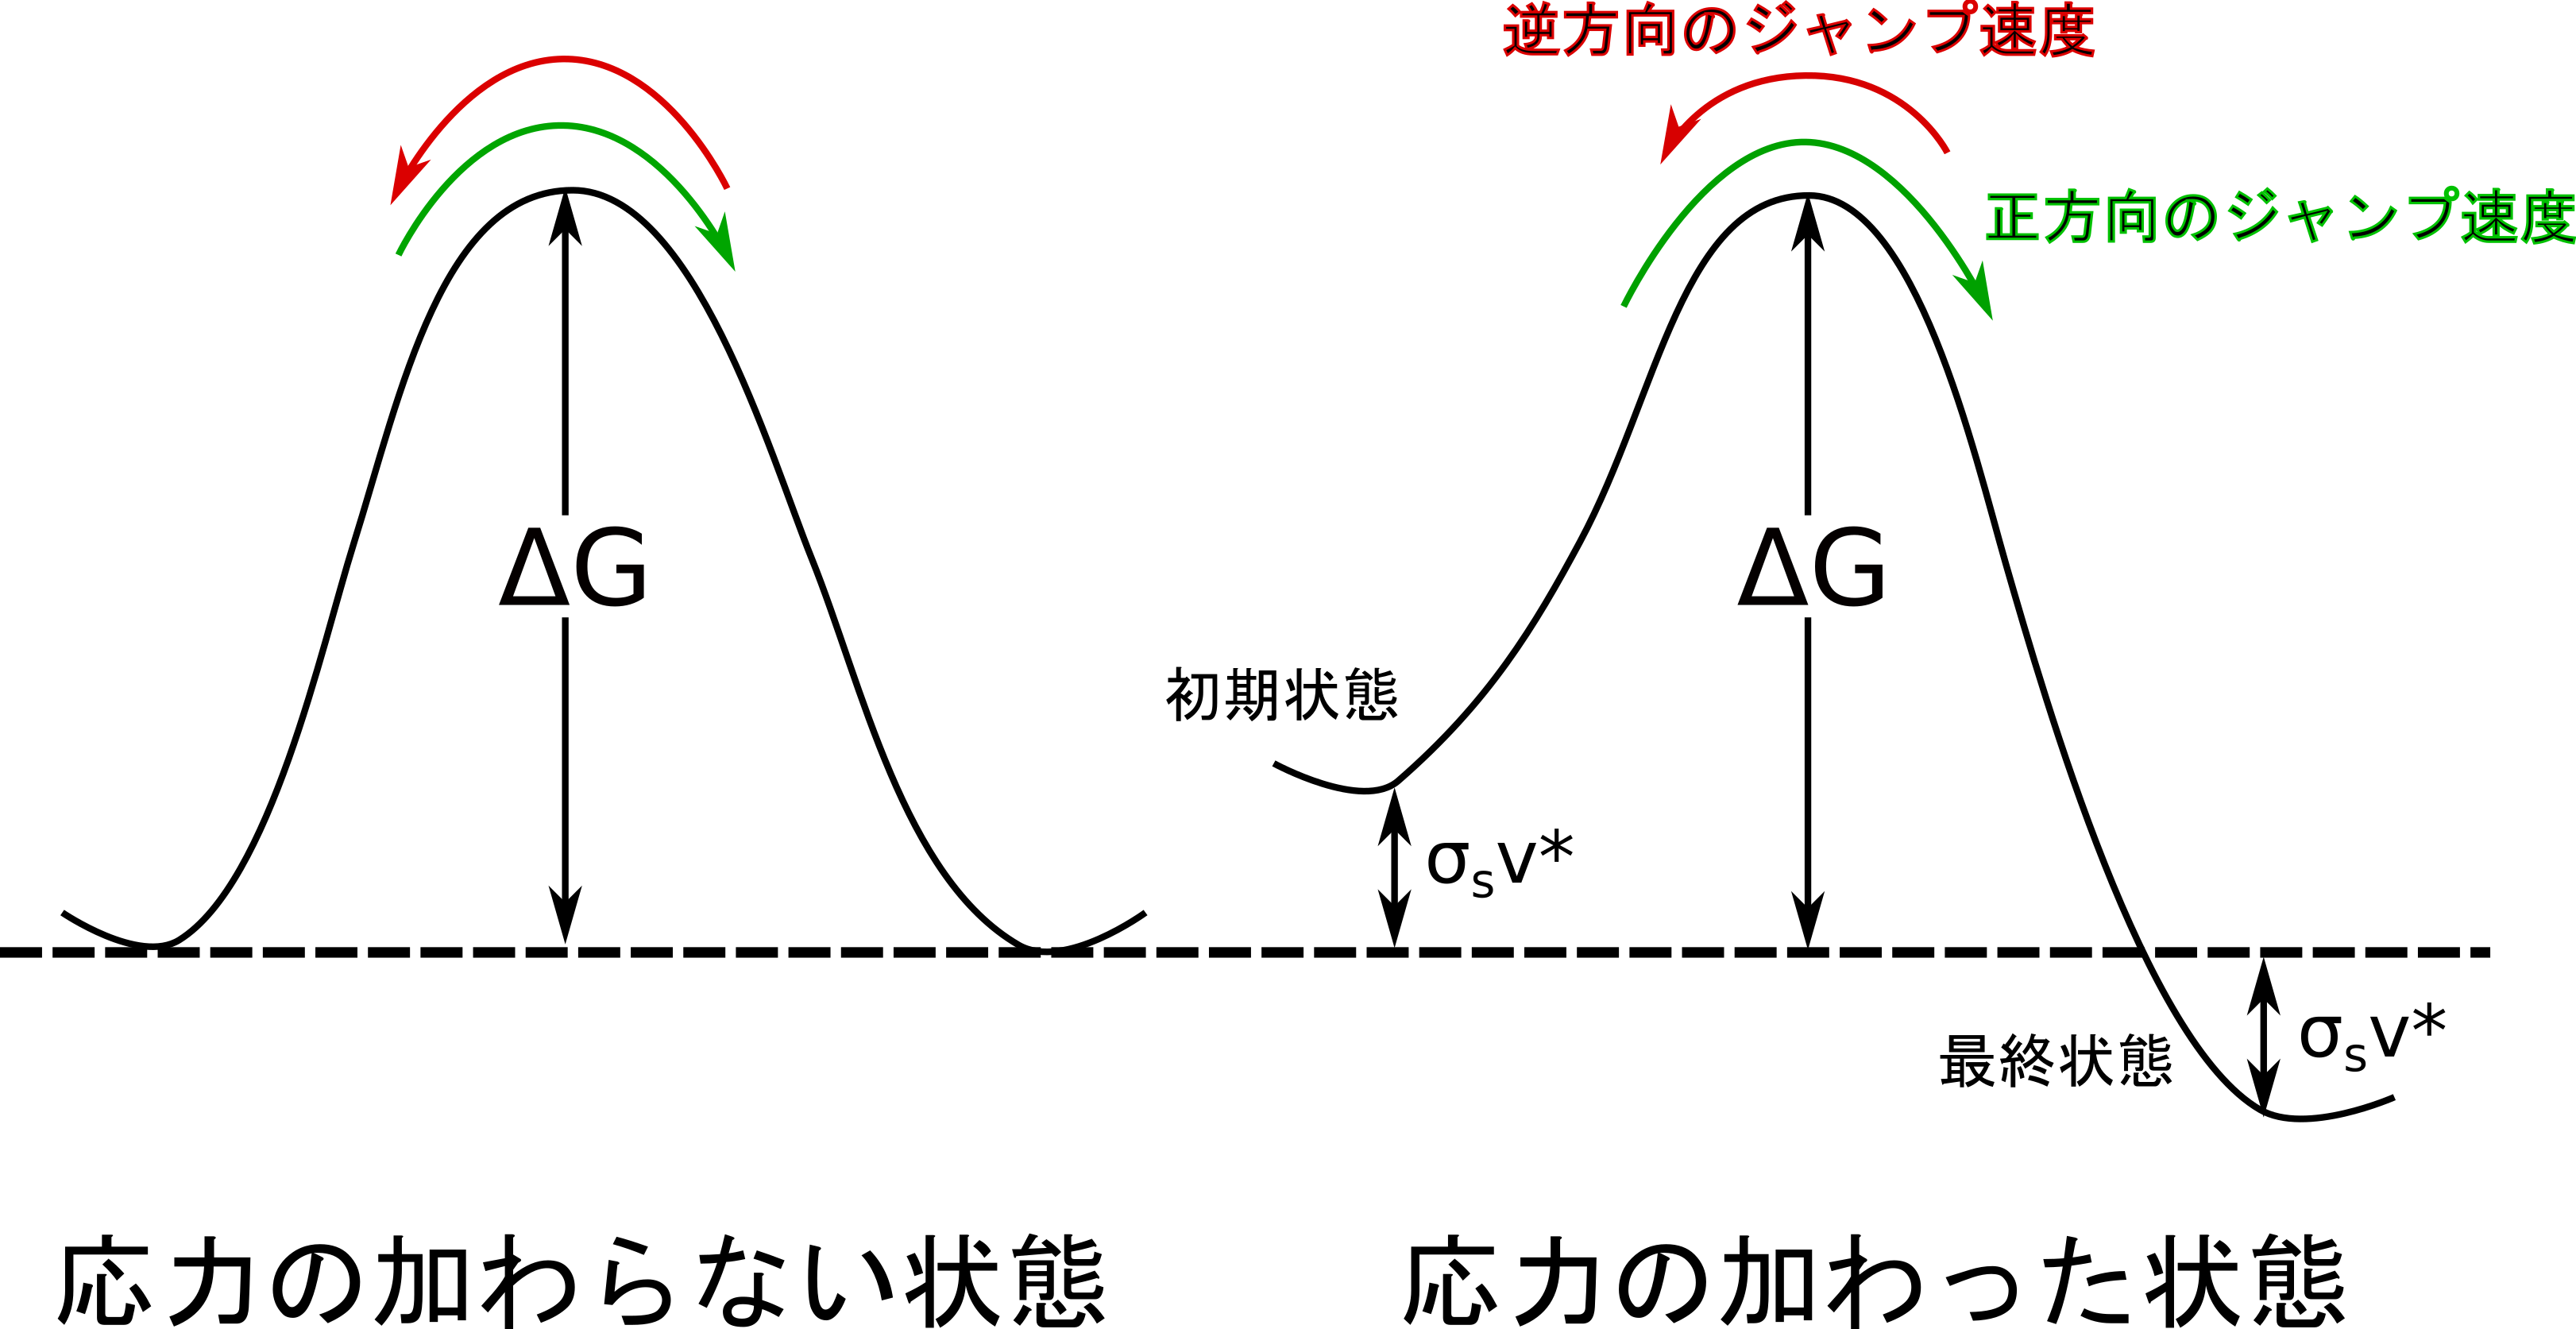
\includegraphics[width=9cm]{flow_under_stress.png}
%	\caption{•}
%	\label{fig: •}
\end{figure}
\end{frame}


%%%%%%%%%

\begin{frame}
\frametitle{Eyring の流動モデル}
    \begin{figure}
    \centering
        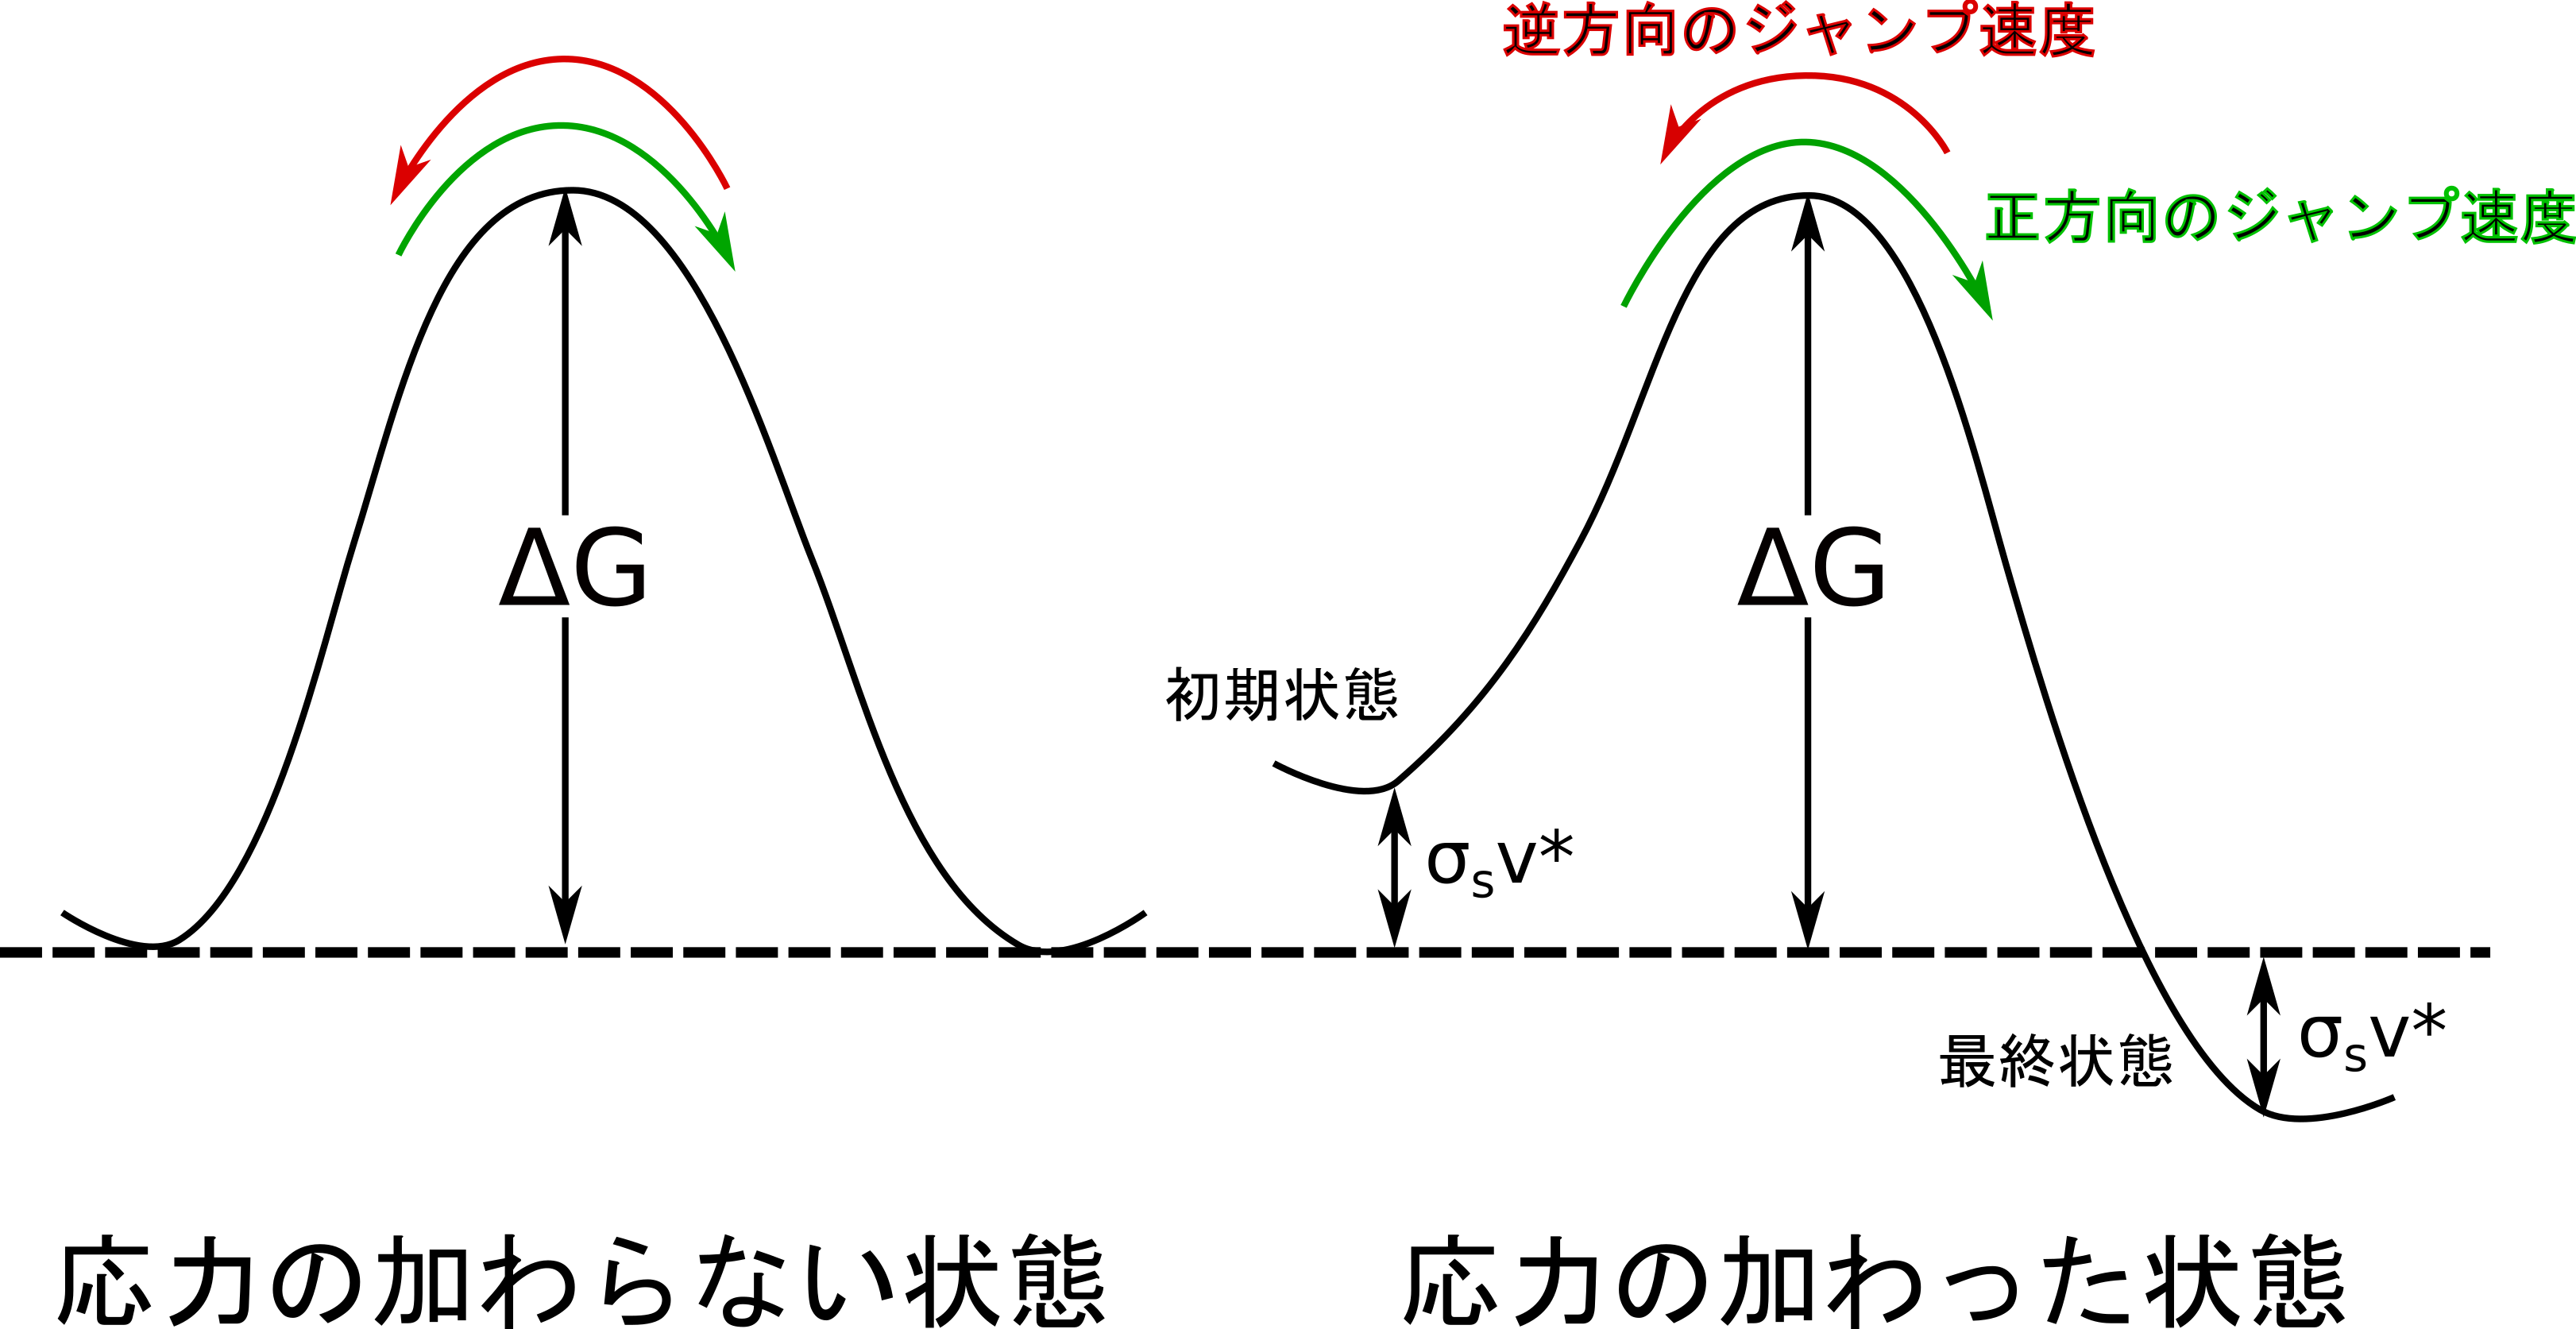
\includegraphics[width=.5\textwidth]{flow_under_stress.png}
    \end{figure}
    \footnotesize
    \begin{columns}[totalwidth=.8\textwidth]
    \column{.5\textwidth}
            \begin{align*}
            R_0 = R_f = R_r = \alpha k_B T \exp \left( - \dfrac{\Delta G}{RT} \right)
            \end{align*}

    \column{.5\textwidth}
            \begin{align*}
            \begin{cases}
    %		\text{応力印加方向} \\
            R_f = \alpha k_B T \exp \left( - \dfrac{\Delta G - \sigma_s v^*}{RT} \right)\\[12pt]
    %		\text{逆方向} \\
            R_r = \alpha k_B T \exp \left( - \dfrac{\Delta G + \sigma_s v^*}{RT} \right)
            \end{cases}
            \end{align*}
	\end{columns}
	
	\begin{align*}
	\alpha = \dfrac{1}{h} \dfrac{F^{\ddag}}{F_0^{\ddag}} 
	\end{align*}
	$h$ はプランクの定数、$F^{\ddag}, F_0^{\ddag}$ は、それぞれ、励起状態及び基底状態の分子の分配関数
\end{frame}



%%%%%%%%%
\begin{frame}
\frametitle{Eyring の流動モデル}
\Large
応力 $\sigma_s$ が印加された場合、\\セグメント(体積 $v^*$ )の移動速度 $R$ は、
\small
\begin{align*}
	R
	&= R_f -R_r \\
	&= \alpha k_B T \exp \left( - \dfrac{\Delta G - \sigma_s v^*}{k_BT} \right)
	-\alpha k_B T \exp \left( - \dfrac{\Delta G + \sigma_s v^*}{k_BT} \right) \\
	&= \alpha k_B T \exp \left( - \dfrac{\Delta G}{k_BT} \right) \exp \left(\dfrac{\sigma_s v^*}{k_BT} \right)
	- \alpha k_B T \exp \left( - \dfrac{\Delta G}{k_BT} \right) \exp \left(\dfrac{-\sigma_s v^*}{k_BT} \right)\\
	&= \alpha k_B T \exp \left( - \dfrac{\Delta G}{k_BT} \right) \left\{ \exp \left(\dfrac{\sigma_s v^*}{k_BT} \right)
	- \exp \left(\dfrac{-\sigma_s v^*}{k_BT} \right) \right\} \\
	&= 2 \alpha k_B T \exp \left( - \dfrac{\Delta G}{k_BT} \right) \sinh \left(\dfrac{\sigma_s v^*}{k_BT} \right)
\end{align*}

\end{frame}


\subsection{ソフトマターの非線形挙動}
%%%%%%%%%
\begin{frame}
\frametitle{アンドレードの粘度式}
\large
%$x \ll 1 \rightarrow \sinh(x) \simeq x$ であるので、
印加応力が非常に小さいか、粒子が小さいとき、分母の熱ゆらぎに比べて分子が非常に小さいとみなせて、
\begin{align*}
& \dfrac{\sigma_s v^*}{k_BT} \ll 1 \rightarrow \sinh(x) \simeq x \\
\therefore &\;  R \simeq 2 \alpha k_B T \exp \left( - \dfrac{\Delta G}{k_BT} \right) \dfrac{\sigma_s v^*}{k_BT}
	=2 \alpha \exp \left( - \dfrac{\Delta G}{k_BT} \right) \sigma_s v^*
\end{align*}

\large
上式中の $R$ は単位時間あたりの粒子の移動量\\
そこで、
$R$ をずりせん断速度 $\dfrac{R}{v^*} = \dot{\gamma}$ とみなせば、\\
$\eta = \dfrac{\sigma}{\dot{\gamma}}$ より
\end{frame}

%%%%%%%%%
\begin{frame}
	\frametitle{アンドレードの粘度式}
	\large
	アンドレードの粘度式である下式を得る。
	\begin{align*}
	\eta = A \exp \left(\dfrac{\Delta G}{k_BT} \right)
	\end{align*}
	
	\large
	これは、粘度が応力に依存しないというニュートン流動を表している。
	
	\end{frame}
%%%%%%%%%
\begin{frame}
\frametitle{ソフトマターの非線形性}
\large
印加応力が大きい、移動する粒子が大きい場合、
\normalsize
\begin{align*}
\dfrac{\sigma_s v^*}{k_BT} \gg 1 \Rightarrow \exp(x) \\
\therefore \; R \simeq 2 R_0 \exp \left( \dfrac{ \sigma_s v^*}{k_BT} \right)
\end{align*}
\large
となり、応力に依存した非線形性が生じる。

\begin{alertblock}{ソフトマターの非線形応答}
一般に、高分子材料等を構成するセグメントは、\\
十分に大きな排除体積を有するので、非線形応答
\end{alertblock}

\end{frame}

%%%%%%%%%%%%%%%%%%%%%%%%%%%%%%%%%%
\subsection{降伏挙動のミクロなモデル}

%%%%%%%%%%%%%%%%%%%%%%%%%%%
\begin{frame}
\frametitle{降伏挙動のモデル}

\Large
\begin{exampleblock}{ミクロな降伏挙動のモデル}
\begin{itemize}
\item
応力印加による局所的な流動
\item
Eyring の流動モデル
	\begin{itemize}
	\large
	\item
	活性化エネルギー($\Delta G$)の山を超えて、\\粒子が移動
	\item
	応力がなければ、両方向の移動が同一
	\item
	応力印加により、移動の不均一(流動)
	\end{itemize}
\end{itemize}
\end{exampleblock}
\end{frame}

%%%%%%%%%%%
\begin{frame}
\frametitle{降伏応力とせん断速度}

\large
移動速度 $R$ を引っ張り変形速度 $\dot{\epsilon}$ とみなし、\\ $\dot{\epsilon}_0$ を定数として以下の関係が示せる。
\normalsize
	\begin{align*}
	\dot{\epsilon} 
	&= \dot{\epsilon}_0 \exp \left( - \dfrac{\Delta G}{RT} \right) 
		\exp \left( \dfrac{ \sigma_s v^*}{RT} \right) \\
	\therefore \; \dfrac{\sigma_s}{T} 
	&= \dfrac{1}{v^*} 
		\left[
			\dfrac{\Delta G}{T} 
			+ R \ln 
			\left(
			\dfrac{\dot{\epsilon}}{\dot{\epsilon}_0} 
			\right) 
		\right] 
	\propto \log \dot{\epsilon}
	\end{align*}

\large

この関係は、ガラス転移温度以下での降伏値の挙動を記述できる。
\end{frame}

%%%%%%%%%%%
\begin{frame}
\frametitle{マクロな降伏値との整合性}


\begin{columns}[totalwidth=1\textwidth]
\column{.4\textwidth}

\begin{block}{実測データとの整合}
ポリカーボネートの降伏値のひずみ速度依存性を、各種温度で実測。

以下の関係が成立。
\begin{align*}
\dfrac{\sigma_s}{T} 
	\propto \log \dot{\epsilon}
\end{align*}
\end{block}
\column{.58\textwidth}

	\begin{figure}
	\centering
	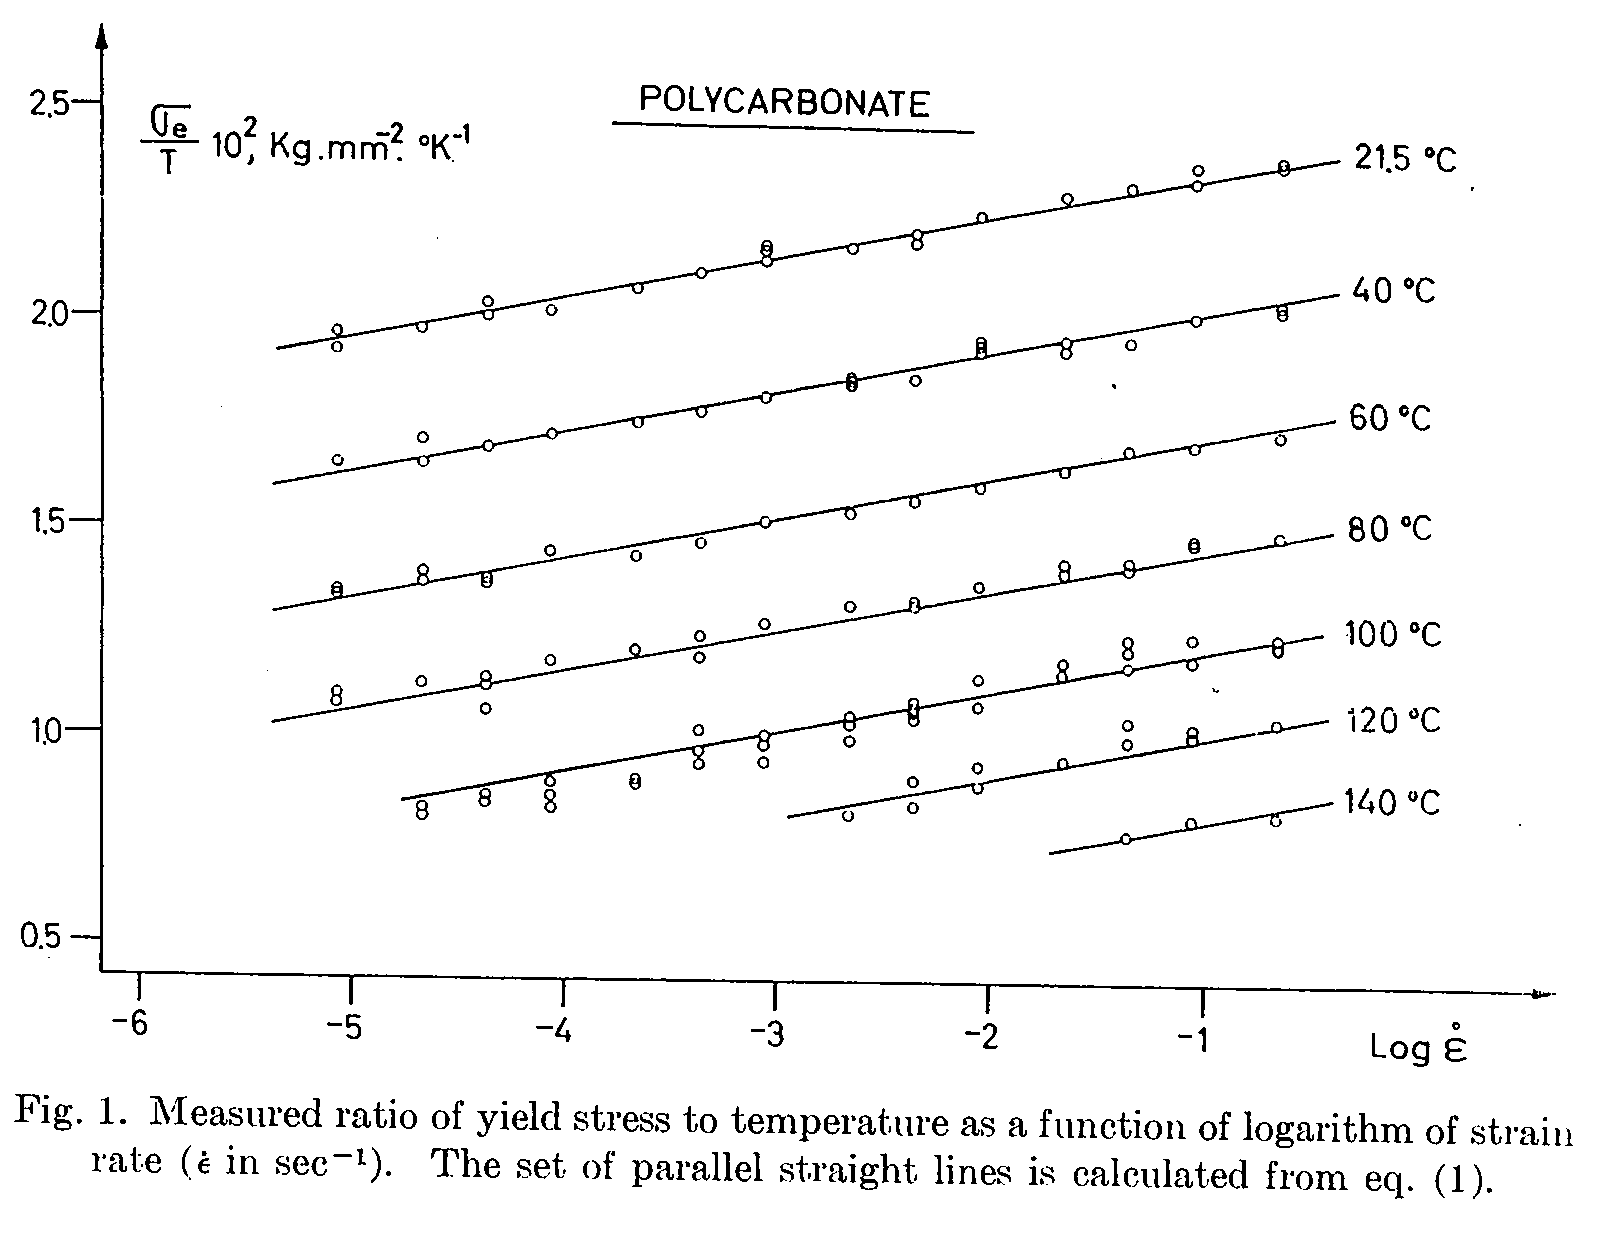
\includegraphics[width=\textwidth]{fig2.png}
	\end{figure}
%\vspace{-1mm}	
%\color{red}チェーンの弱いところが\\壊れる
%

\end{columns}
Bauwens-Crowet, C., Bauwens, J. C., \& Homès, G. \\
``Tensile yield-stress behavior of glassy polymers.''\\
Journal of Polymer Science Part A-2, 7(4), 735 (1969). 
\end{frame}


\begin{frame}
	\frametitle{接着の統計モデル}
	\begin{itemize}
		\item 接着状態の評価
		\begin{itemize}
			\item 接着したサンプルに外力を印加し、破断する値を接着強度とする
			\item その接着状態を最もよく表す荷重近傍で破壊し、その値の周辺に散らばる。
		\end{itemize}
		\item 良好な接着状態
		\begin{itemize}
			\item 凝集破壊モードの場合、比較的揃った値で破断する。
			\item かつての原賀氏の実験結果によれば、その散らばり具合は正規分布かのように見える。←確率紙で判断
		\end{itemize}
		\item この散らばりを誤差と考えれば左右対称での違和感はないが、
		\item 本当に対称で妥当なのだろうか?
	\end{itemize}
\end{frame}

% \begin{frame}
% 	\frametitle{接着強度の分布関数}
% 		\begin{itemize}
% 			\item 実務的には、大きい側に伸びたロングテールは問題ない。
% 			\item 0の方に伸びた分布の0近傍の小さいところでの振る舞いが大事かもしれない。
% 			\item そもそも接着強度に負の値はない。⇔単純な正規分布はおかしい。
% 			\item 正の値の連続値の分布関数
% 			\begin{itemize}
% 				\item \href{https://en.wikipedia.org/wiki/Weibull_distribution}{ワイブル分布}
% 				\item \href{https://en.wikipedia.org/wiki/Gamma_distribution}{ガンマ分布}
% 				\item \href{https://ja.wikipedia.org/wiki/%E5%AF%BE%E6%95%B0%E6%AD%A3%E8%A6%8F%E5%88%86%E5%B8%83#:~:text=%E7%A2%BA%E7%8E%87%E8%AB%96%E3%81%8A%E3%82%88%E3%81%B3%E7%B5%B1%E8%A8%88%E5%AD%A6,%E3%82%82%E3%81%AE%E3%81%A8%E3%81%97%E3%81%A6%E5%AE%9A%E7%BE%A9%E3%81%95%E3%82%8C%E3%82%8B%E3%80%82}{対数正規分布}
% 			\end{itemize}
% 		\end{itemize}
% \end{frame}

% \begin{frame}
% 	\frametitle{Rの導入}
	
% \end{frame}

\end{document}